\documentclass[]{Learning-to-Play-Wolfenstein-thesis}
\usepackage{graphicx}
\usepackage{hyperref}
\usepackage{amssymb}


%%%%%%%%%%%%%%%%%%%%%%
%%% Input project details

\def\studentname{Gear\'oid N\'i Ghiolla Coinnig} % Edit with your name
\def\projecttitle{Learning to Play Wolfenstein3D} % Edit with you project title
\def\supervisorname{Prof. Arthur Cater}


\begin{document}

\maketitle

%%%%%%%%%%%%%%%%%%%%%%
%%% Your Project Specification

\chapter*{Project Specification}
\fontsize{12pt}{21pt}{\textbf{General Information:}}\\\\
The goal is to develop a program able to play some early stages of the first person shooter video game "Wolfenstein", by learning to associate possible actions (moving in various ways, shooting) with what is perceptible in the game at any moment. A technique that proved successful in learning to play a Mario Bros level is to be applied to the new game. An existing open-source reimplementation of Wolfenstein will need to be adapted to provide the learner with information about what it perceives, where it is, how much ammunition it has, and how much time has elapsed.\\

The technique to be used for learning to play is a combination of neural network and genetic programming. Input neurons correspond to the presence of visible or measurable features (walls, enemies, power-ups, clock), and output neurons correspond to controller buttons (go left/right/forward/back, turn left/right/upward/downward, jump, shoot). By starting with a minimal network, adding random links from inputs to hidden nodes and onward to output nodes or perhaps other hidden nodes, and randomly adding new hidden nodes, different behaviours are obtained. By applying ideas of genetic algorithms, many individuals can be created and rated in terms of how much progress they make before dying and how soon they die. Mutation of, and crossover among, the more successful individuals of a generation leads over time to general improvement and ultimately, it is hoped, a really excellent player.\\

This technique succeeded in a Mario Bros game level, using inter-neuron links that had simple weights: excitatory or inhibitory. The Wolfenstein game has several similar characteristics, being deterministic and possessing something that can be used as a measure of progress (in Mario, a combination of distance from start and time taken was used but coins gathered were ignored).\\

\fontsize{12pt}{21pt}{\textbf{Mandatory: }}
\begin{itemize}
\item Install the open-source reimplementation of Wolfenstein.
\item Identify and implement code changes necessary to determine whether the hero has died, and if so, at what time and distance from starting.
\item Identify and implement code changes necessary to allow a program rather than a human to control the character's actions.
\item Identify and implement code changes necessary to allow a program to detect what is visible to the character at any moment in play.
\item Design and implement a system for linking measurements of what can be detected in several of the floors of the first stage of Wolfenstein to activation of the player controls, using a small randomly generated system of neurons (nodes) and links that are either excitatory or inhibitory. (Such a system is virtually certain to die quickly.) Only small numbers of links in to or out from any node should be permitted at this stage, a maximum of six.
\item Develop a way to combine parts of one random network with parts of another.
\end{itemize}
\newpage
\fontsize{12pt}{21pt}{\textbf{Discretionary: }}
\begin{itemize}
\item Design and develop a metric for comparing the degree of success of two networks, in terms of (large) distance travelled and (fast) time taken.
\item Design and develop an evolutionary mechanism for taking a generation of several individual networks, picking the best few, performing crossovers and occasional mutations (new hidden nodes, wholly new links) in order to create a new generation of individuals.
\item Apply this mechanism for at least 20 generations each consisting of at least 12 individuals. Measure the performances of the best, worst and median individuals in each generation.
\item Apply the entire system to a third of the levels in the first Stage of Wolfenstein.
\end{itemize}

\fontsize{12pt}{21pt}{\textbf{Exceptional: }}
\begin{itemize}
\item Apply this mechanism to substantially more generations, or substantially larger generations, or with more generous limits on in-degree and out-degree of nodes. Measure performance.
\item Enrich the measure of performance, for example to reward the kills of enemies and the low use of ammunition.
\item Apply the entire system to half or more of the levels in the first Stage of Wolfenstein.
\end{itemize}
%%%%%%%%%%%%%%%%%%%%%%
%%% Your Abstract here

\begin{abstract}
Wolfenstein3D is a first person shooter MS-DOS game that was released in 1992. The goal of the video game is to escape Castle Wolfenstein, a Nazi prison. Its creators, ID Software, released the source port for the game in 1995 meaning it is now possible to edit the source code for our own purposes.

The aim of the \textit{Learning to Play Wolfenstein3D} project is to replace a human player with a computer that progressively learns to play Wolfenstein3D using two Artificial Intelligence concepts, Genetic Programming and Neural Networks. These algorithms are implemented according to an algorithm called \textit{NeuroEvolution of Augmenting Topologies (NEAT)} which is based off a paper written by Kenneth Stanley and Risto Miikkulainen. Henceforth, the AI bot created as a result of this project shall be dubbed NEATDoop (A Developing Object-Orientated Program, also because I like the name NEATDoop)

NEATDoop's learning process will be aided by a weighting function that measures the success of a particular attempt that it has made at playing the game which is a requirement for any project of this nature. By using previous attempts a new, hopefully better, attempt at playing the game will be generated. The end goal being that NEATDoop is a fully functioning AI that is capable of learning how to play some levels of the Wolfenstein3D campaign
\end{abstract}
\newpage


%%%%%%%%%%%%%%%%%%%%%%
%%% Acknowledgments

\chapter*{Acknowledgments}

I wish to express my sincere gratitude to the various community forum pages that have aided me in setting up such a strong foundation for my project. These include but are not limited to the DoomWorld forums, DRD team forums, StackOverflow, Wolfenstein3D Dome and the Wolf3D haven forums.

I would like to personally thank Iona Chera for providing me with information and feedback on my initial project concepts. I'd also like to thank him for outlining various ways in which I could work with the source code for Wolfenstein3D.

I want to thank my fellow classmates Joe Duffin and James Keating for always finding the time to help me with problems I have had with my project. Without their help I fear that this project may not have been as complete as it is to date.

Finally I would like to thank my supervisor Prof. Arthur Cater. Over the past year he has continually provided me with support and feedback on my project and I cannot thank him enough for that.
%%%%%%%%%%%%%%%%%%%%%%
%%% Table of Content

\tableofcontents\pdfbookmark[0]{Table of Contents}{toc}\newpage
\newpage


%%%%%%%%%%%%%%%%%%%%%%
%%% Introduction
\chapter{Introduction}

\chapter{Background Research}	% talk about what was seen in prev chapter at start
This chapter will outline in detail the discoveries that were made whilst researching numerous relevant topics of interest to the \textit{Learning to Play Wolfenstein3D} project. The first item that will be discussed will be the game selection process; what caused Wolfenstein to be chosen over previously considered open-source games, such as Doom and Duke Nukem. However, the main topic of discussion in this chapter will be the \textit{NeuroEvolution of Augmenting Topologies(NEAT)} algorithm; what it is and why it will be of major importance to NEATDoop's ability to learn.


\section{Game Selection}
In order for an AI to be able to learn to play Wolfenstein it will need to be able to make decisions based on what it can see at any point in time. This would not be possible for a game whose code was not open source since it would be impossible for the AI to read from the source code to determine what its surroundings are composed of.

The first open source game that was considered for this project was \textit{Duke Nukem 3D}. It was released early 1996 and was developed by \textit{3D Realms}. The game was discovered having read an analysis of the games source code on a web-blog early into the specification for this project. REF[3] 

Having contacted the author of the web-blog and discussed the project idea, he recommended that I do not use \textit{Duke Nukem 3D} due to its ”rotten codebase”. From inspection of an open source implementation of the source code called \textit{Chocolate Duke Nukem 3D} the authors recommendation seemed well founded. The source code itself is rather immense and is very, very sparingly documented. By comparing the game.c source file from \textit{Duke Nukem 3D} and the WL\_GAME.c source file from Wolfenstein it is now very clear that not choosing \textit{Duke Nukem 3D} was a solid decision. Both of these source files implement logic that sets up levels, constructs in game text, displays player health statistics and includes logic that is fundamental to the main game loop. WL\_GAME.c from \textit{Wolfenstein’s} source port is contains approximately 1,600 lines of code whereas game.c from \textit{Duke Nukem 3D’s} source port alone roughly contains 11,000 lines of code with no substantial documentation indicating how the source file works. REF[4] [5]

\textit{The Original Doom} was then considered as it was recommended by the author of the previously mentioned web-blog. Having contacted a software developer who created an implementation of the Doom source port called \textit{AutoDoom} REF[6] he recommended that \textit{Wolfenstein 3D} be considered for this project as opposed to Doom due to the fact that Doom’s level design is a lot more complex than Wolfenstein’s. This is evident from any gameplay showcasing the games. REF[7] [8] 

\textit{Doom} allows for players to move in the vertical axis. This extra dimension that a player can move in would have been a huge roadblock in NEATDoop’s ability to learn. \textit{Wolfenstein’s} map design is completely flat i.e. the player cannot move in the vertical axis. A worst case scenario for NEATDoop playing Wolfenstein is that it gets stuck in a corner or runs in a circle. Not only would this be a concern in Doom but there exists a probability that NEATDoop would get stuck behind a staircase or similar. The fitness function for Doom would also have to take into account the extra axis which would have resulted in an even more complex measure of fitness.

As a result of the outlined problems, Wolfenstein was chosen for this project because the source port is well documented. As well as this the source port, whilst still relatively large, is pretty easy to navigate and understand. The source port that was chosen is actually not the original one that was written in C but an alternative version written in C++ called Wolf4SDL. The reason behind this was mainly so any code written to interact with the Wolfenstein source code could be object oriented. Further reasons will be discussed later in Chapter~\ref{Chapter3}.

\section{Wolfenstein 3-D Game Mechanics}
By the very nature of this project it is of high importance to be able to understand the source code of the game in order to determine what information can and cannot be used for NEATDoop's learning. This section will introduce how Wolfenstein's gameplay works and also give a brief description on some parts of the source code where attention was  focused early on. The goal of reading the source code at this stage was to understand how the Wolfenstein map is represented and how objects, such as enemies and pickups, are tracked throughout gameplay. These components will form an important base for the NEAT algorithm which is discussed after this section.

\subsection{Wolfenstein's Gameplay}
Wolfenstein is a First-Person Shooter(FPS) and the goal of the each level is to get to an elevator tile that brings the character to the next level. A player reaches the end of each level by moving through a series of rooms in the game, potentially killing enemies and picking up items such as health, ammo, treasure or new guns as it does so. 

Depending on the difficulty selected, a variety of enemies will spawn in the game. These enemies will attempt to kill the player on sight. The player is equipped with a low-power pistol and a knife by default, although it is possible to pick up a sub-machine gun or a chain gun in various levels that offers a higher damage output than the pistol. 

Damage is done on a distance basis. The closer you are to an enemy when you hit them, the more damage that is inflicted. This also applies to enemies, the closer they are to you the more damage they do when they hit you. 

Enemies react to sound. On hearing a gunshot, an enemy will move in the direction of the gunshot. As will be seen later, this will be the cause of a substantial amount of deaths in NEATDoop's learning where it shoots randomly and attracts enemies that ultimately, kill it.

\subsection{Map Representation}
Every map in Wolfenstein is represented as a 64x64 grid of tiles. It holds \textit{Byte} values indicating the type of structure located at that (x,y) co-ordinate. If the \textit{Byte} value at a particular (x,y) co-ordinate is greater than 0, then it can either be a wall, push-wall, door or an elevator tile (which is the tile associated with the end of the current level). If the value at any (x,y) co-ordinate is 0 then it represents a tile that a player can walk on.

This particular information is incredibly important for determining the structural surroundings of NEATDoop during gameplay. From this \textit{2 dimensional array of bytes} we can get the spawn location in each level, the end location in each level and all wall, door and push-wall data that will be used primarily as input to the neural networks that will be described later. 

The \textit{elevator tile} is a particularly important tile. On this tile a button is located that, when pressed by the player, ends the current level. The co-ordinates of this tile position will be used later in the fitness function as will the spawn co-ordinates. 

\subsection{Enemy/Item Representation}
Both enemies and items that can be picked up are represented as \textit{structs} within the source code. 

So called \textit{Actors}, represent enemies and the player of the game. The \textit{struct} storing their information is named \textit{objstruct} and contains information about the position of the Actor in the map, the health the Actor has, the sprite image assigned to it and references to the next and previous \textit{objstruct} etc. A list of objstructs is maintained with the name \textit{objlist} which stores all Actors currently alive on the map.

Items that can be picked up include things like guns, ammo, health and treasure. These are considered to be \textit{static items} in the Wolfenstein Engine since they do not move. However, other items such as chairs, tables and statues are also considered to be static. The \textit{struct} that represents these static objects is called \textit{statstruct} and a list maintaining references to all static items currently on the map is called \textit{statobjlist}.

Identifying static items of interest is rather simple since each static item has a label associated with it. For instance, ammo has a \textit{bo\_clip} label associated with it so it is possible to iterate through the \textit{statobjlist} array and find items that would be considered useful for NEATDoop to pickup. 
\newpage
\section{NEAT Algorithm}
NEAT stands for \textit{Neuro-Evolution of Augmenting Topologies} and is based on an paper by Kenneth Stanley and Risto Miikkulainen~\cite{NEAT:2002}. The paper demonstrates the ability for the NEAT algorithm to solve problems in quicker succession than other types of topology evolving algorithms such as \textit{Topology and Weight Evolving Artificial Neural Networks (TWEANN)} algorithms. The NEAT algorithm consists of two very important Machine Learning techniques, Neural Networks and Genetic Algorithms.\\\\

			
\subsection{\label{}NEAT Neural Networks}
Neural Networks(NN) are a Machine Learning technique that roughly simulate the behaviour of a brain. They generally consist of artificial Neurons that are connected using artificial Synapses. The synapses in a NN typically have a weight associated with them that describes how strong a connection any two neurons have with each other.

In traditional Neuroevolution techniques, a topology is chosen before any experimentation begins. This topology is normally maximally connected, meaning that every input is connected to every hidden / output unit and every hidden unit is connected to every output unit. The network is then modified by means of mutating the weights on these links using evolutionary techniques such as genetic algorithms. The goal of this type of neuroevolution is therefore to optimise the weight matrix associated with the network.

In order to determine what Neurons are active at any point during network analysis, an \textit{activation function} is used. In NEAT, a modified Sigmoidal transfer function is used, {$\varphi(x) = \frac{1}{1 + e^{-4.9x}}$}. This steepened sigmoid allows more fine-tuning at extreme activations. It is defined to be close to linear at its steepest ascent between activations -0.5 and 0.5. ~\cite{NEAT:sigmoid}

\begin{figure}[h]
\centering
\fboxsep 2mm
\framebox{
	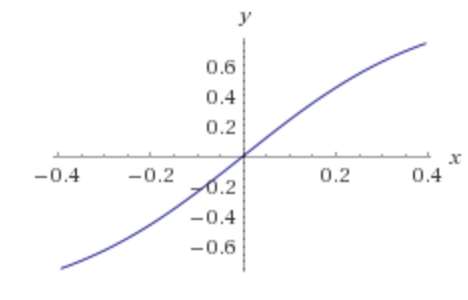
\includegraphics[width=6cm]{sigmoid} 
}
\caption{\label{fig:NEAT_sigmoid} Modified Sigmoidal activation function used for NEAT algorithm}
\end{figure} 
The weights between Neurons are not the only aspect of a Neural Network that contribute to their behaviour. The structure of a neural network also affects its functionality. The NEAT algorithm is primarily focused on this aspect of neuroevolution. It extends and tries to improve on some popular techniques utilised by some TWEANNs. The two main ideas it introduces are the \textit{Speciation} of a population and using \textit{Innovation Numbers} on network encodings so that the historical origins of each network can be tracked. These concepts try to counter some of the common issues with typical TWEANNs.\\

\subsubsection{NEAT Encoding}
Typical neural networks consist of Neurons (nodes) connected using Synapses (links). NEAT describes its networks using a type of direct encoding whereby each network is represented using a series of \textit{Genes}. Each Gene indicates two Neurons that are connected, whether or not the link is enabled, a weight and an \textit{innovation number} that is unique to each Gene. This innovation number is used to calculate similarities between networks.

\begin{figure}[h]
\centering
\fboxsep 2mm
\framebox{
	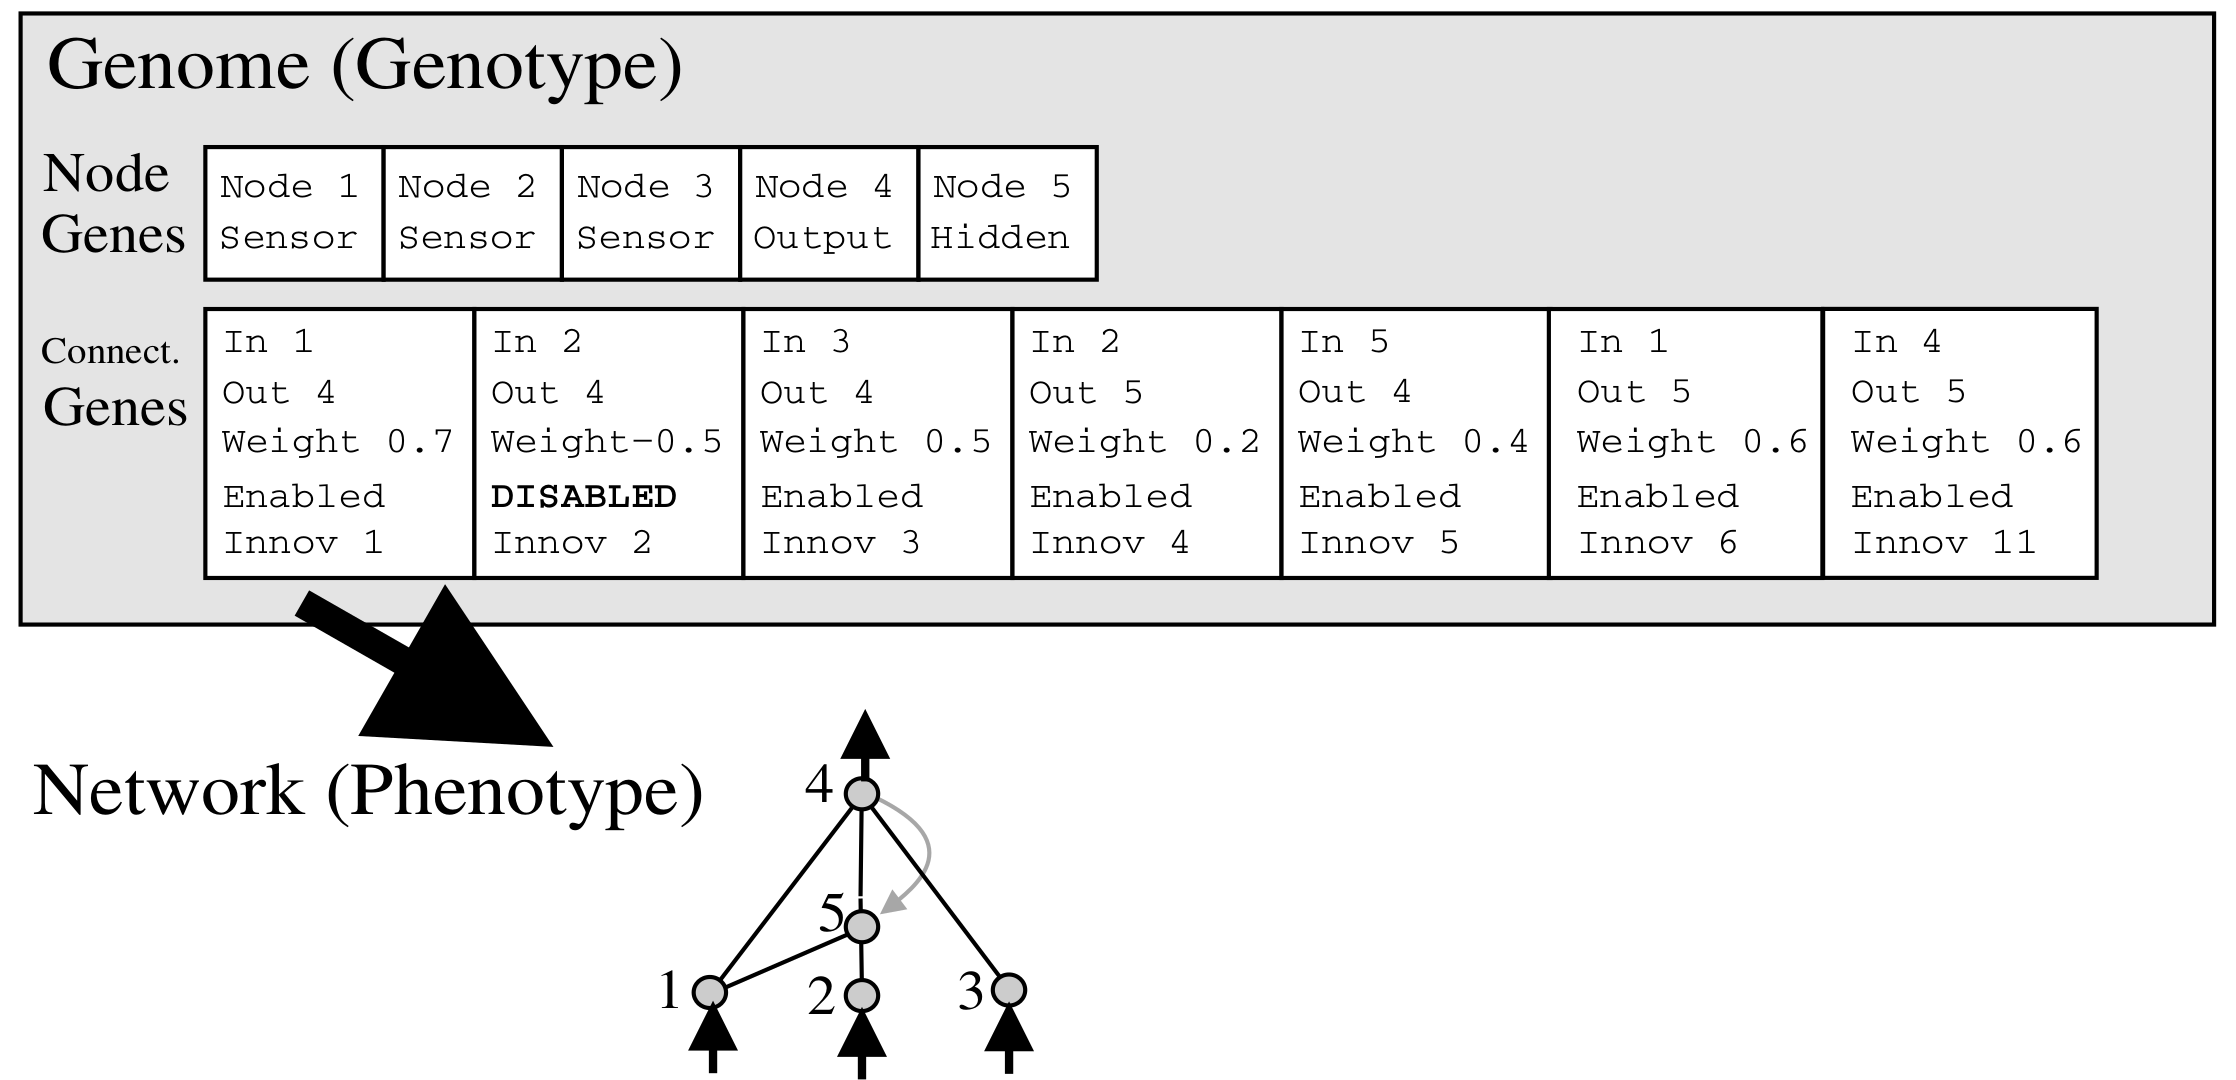
\includegraphics[width=14cm]{encoding} 
}
\caption{\label{fig:NEAT_encoding} Genotype to Phenotype example mapping, where a Gene represents links between Neurons in the Network.}
\end{figure} 
Fig 2.2 is taken directly from the NEAT paper and indicates what a typical genotype to phenotype mapping might look like. Notice that the innovation numbers associated with each Gene in this network are not increasing uniformly. This is an example where Genes would have have been added to another network before the last Gene in this Genome's genotype was added.~\cite{NEAT:encoding}

\subsubsection{\label{subsection2.3.1}NEAT Speciation}
Many problems arise when experimenting with networks that involve modifying the structure of the network as well as the weights on links in order to produce better offspring. One such problem is that, in many cases, modifying a network causes an initial decrease in genotype fitness. As a result, the topological innovation is very unlikely to make it through to the next generation where it has the potential to be optimised. 

In order to counter the above problem the NEAT algorithm uses speciation on its population. This is done by grouping Genotypes by their Phenotypes if they share similar enough genetic history. 

\begin{figure}[h]
\centering
\fboxsep 2mm
\framebox{
	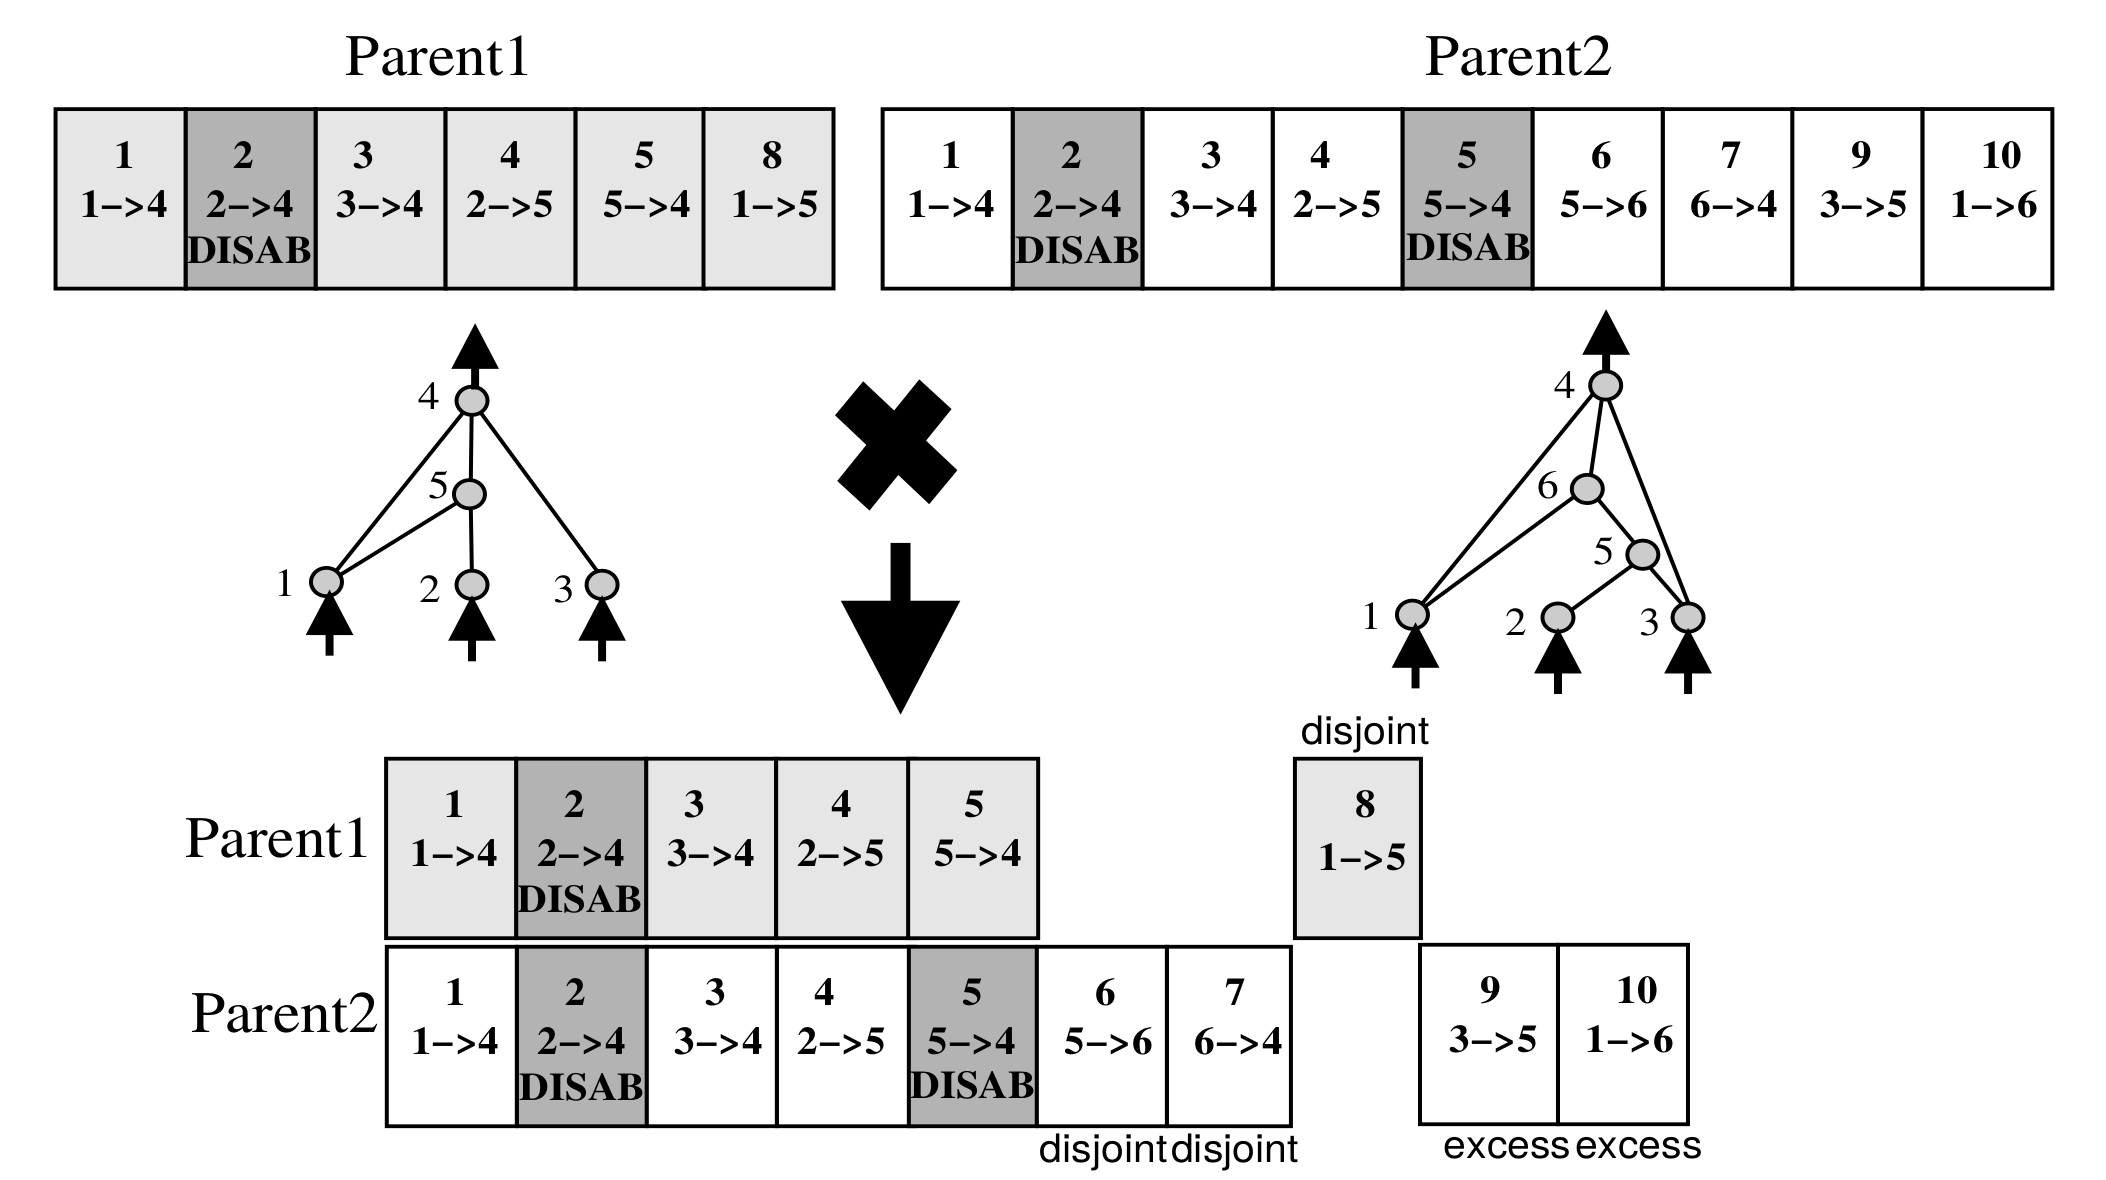
\includegraphics[width=12cm]{neat_innovation} 
}
\caption{\label{fig:NEAT_innovation} Showing a comparison of two Genotypes by examining their shared genetic history i.e. their shared Genes}
\end{figure} 

Figure 2.3 shows an example as to how comparing genetic history might work. The Genes that appear in both individuals are lined up. These Genes are referred to as \textit{Matching Genes}. Any Genes that do not match are considered to either be \textit{Disjoint} or \textit{Excess} depending on whether the mismatch appears in the middle of the comparison or at the end. This method for computing Genotype similarities will be useful later when NEAT genetic algorithms are introduced the next section. ~\cite{NEAT:speciation}

There are a number of implications of Speciation. Firstly, structural innovations have a better chance of making it through to the next generation where they can be further optimised. Secondly, it reduces the chances of a single Genome from dominating the entire population. 

Speciation is a concept that most TWEANNs do not employ, as indicated in the NEAT paper. Innovative structures in TWEANNs tend to have more connections and as such take far longer to optimise than simpler ones. The result of this is that innovative structures in TWEANNs cannot compete with simpler ones.

\subsection{\label{section2.5}NEAT Genetic Algorithms}
Genetic Algorithms(GA) are a set of rules that try to describe how simulated evolution might work with an artificial population. The population consists of a set of individuals that are to be subject to these rules of evolution. The individuals are evaluated and their relative success measured according to some \textit{Fitness Function}. Depending on the implementation, a number of individuals are then moved forward to the next generation where the same rules are applied to the new modified population. This process is repeated until a terminal condition is met. In the case of this project the terminal condition will ultimately be NEATDoop completing a level.

The GA used for NEAT is a variation of these standard rules, since the population is \textit{speciated}\textbackslash sub-divided the rules are altered slightly.
\begin{enumerate}
\item\textbf{Initialisation:} As was mentioned in Subsection\ref{subsection2.3.1} the population in the NEAT algorithm is Speciated or sub-divided so that clusters of similar Genotypes are created. This is how the population in NEAT is created. Each Genotype starts with a network that is minimally connected, meaning that there is no hidden layer initially; only an Input and Output layer.
\item\textbf{Evaluation:} This step involves taking each Genotype, feeding it inputs in order to produce some output. The fitness or success of the Genotype is then calculated according to some fitness function which is used as a measure for comparison between Genotypes. 

NEAT uses \textit{explicit fitness sharing} between the Genotypes of a particular niche. This value is assigned the fitness of the highest performing Genotype in that niche. It does this so that no single niche or \textit{Species}, as they are also called, can take over the entire population even if all of its members are high performing.~\cite{NEAT:fitshare}
\item\textbf{Selection:} Once all the Genotypes in the population have been evaluated, niches\textbackslash species reproduce by first eliminating the lowest performing Genotypes and then the entire population is replaced by the offspring of the remaining Genotypes in each niche\textbackslash species. 

In the implementation for this project, only the best Genotype per species is actually brought forward to the next generation. Since all Genotypes in a species are either equal in performance or worse than the current best performer, removing them creates a higher chance that new ones generated will perform better than the current best.
\item\textbf{Crossover:} Producing new offspring for the next generation involves taking two parent Genotypes from the same species and combining aspects of them to produce a child. The parent Genotypes always come from the same species since the phenotypes of each are similar enough for this crossover to work properly. 

If the phenotypes were not similar then too many disjoint and excess Genes would be used in the child causing the genetic history shared to become tainted.
\item\textbf{Mutation:} In order to introduce genetic diversity within the population mutations are performed on the population. Types of mutations include:
\begin{itemize}
\item NEAT Phenotype modifications (Discussed in the next section)
\item Enabling/disabling existing links in a phenotype
\item Modifying Genotype mutation rates
\end{itemize}
\item\textbf{Repeat process until terminal condition met}
\end{enumerate}

\subsection{\label{subsection2.3.3}NEAT Topological Mutations}
NEAT specifies two types of phenotype mutations, \textit{Node mutations} and \textit{Link mutations}. Both of these mutations add new connection Genes to a Genotype and each new Gene is assigned a new unique Innovation Number. ~\cite{NEAT:topmut}
\begin{figure}[h]
\centering
\fboxsep 2mm
\framebox{
	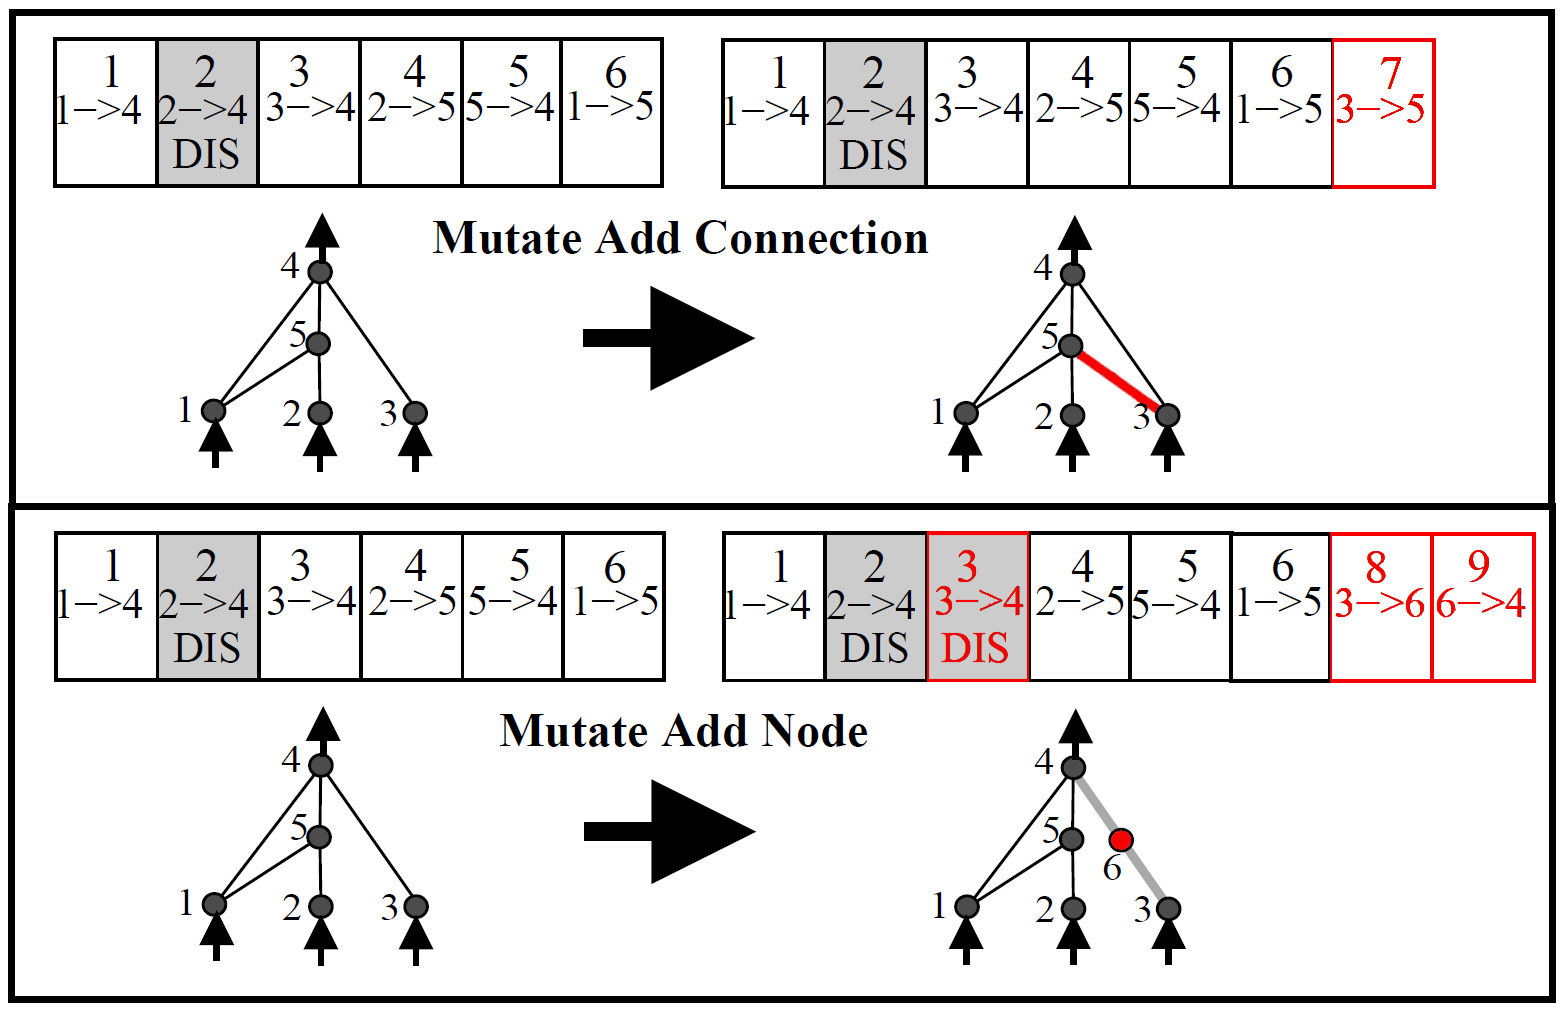
\includegraphics[width=14cm]{neat_mut} 
}
\caption{\label{fig:NEAT_mutations} Shows network phenotypes before and after NEAT Link and Node mutations.}
\end{figure} 
\begin{itemize}
\item\textbf{Link mutation:} In a link mutation a new connection Gene is added to the Genotype specifying an in-neuron and out-neuron. Both of these neurons are chosen randomly from the Genotypes pool of existing neurons. If a link already exists between these two neurons then no new link is added. Fig 2.4 above shows that the neurons selected where 3 and 5 for this specific link mutation example. Notice that the numbers at the top of the displayed diagrams are actually the innovation numbers on each connection Gene.
\item\textbf{Node mutation:} A node mutation involves randomly selecting a Gene from a Genotype. This Gene is then set to be disabled, meaning there is no longer a direct connection between the Gene's in-neuron and out-neuron. Fig 2.4 above shows the Gene selected has 3 as its in-neuron and 4 as its out-neuron. 

Once the selected Gene is disabled, two new connection Genes are created and added to the Genotype.
\begin{itemize}
\item The first Gene has the old in-neuron as its in-neuron and the newly added neuron as its out-neuron (3 -{$\textgreater$} 6)
\item The second Gene has the newly added neuron as its in-neuron and the old out-neuron as its out-neuron. (6 -{$\textgreater$} 4)
\end{itemize}
\end{itemize}

This chapter provides an overview of the work that was done early into the project timeline. Having come to a decision on which game to use, the next natural step was to gain some insight into how the most important information is represented as well as understanding how the mechanics for the game work so that some factors from it could be used later on when designing the fitness function. Finally, the NEAT algorithm was introduced which will be core to the AI's ability to learn.
%talk about what was said and how it relates to next chapter


\chapter{\label{Chapter3}Project Approach}% talk about what was seen in prev chapter at start
The previous chapter introduced the game that was used for this project and outlined the NEAT algorithm, which is at the very core of this project. This chapter will introduce the source port used throughout the project, describe the methods employed in order to identify and understand the most important source files from the Wolfenstein source port and the importance of reading other adaptions of the NEAT algorithm.

\section{Selecting the Source Port}
Wolfenstein 3-D was originally written in a combination of the C and Assembly languages. Very early on in this project it was desired to find another adaption of the Wolfenstein source so that integrating the NEAT algorithm into the source code would not involve writing in either of these languages. This was primarily because the NEAT algorithm is much easier to understand if it is implemented in an Object-Oriented language such as C++. As such, a source port implemented in C++ was sought after. 

Initially the original source port was used. This involved using a compiler known as \textit{Borland C++ v3.1}, which is an old, outdated piece of software, in order to compile to source code. The \textit{Borland} compiler is a 16-bit compiler requiring it to be used within \textit{DosBox}, since it is not possible to run the compiler natively on a 64-bit machine. It was decided eventually that this means of compiling and executing the source code was not ideal and so alternatives were considered.

Since it was desired that a C++ implementation of the source port be used, \textit{WOLF4SDL} was a promising candidate. This particular source port is essentially the same as the original source port but it is commented more generously and allows the possibility for an object oriented language. Compiling the source code was still not ideal with this source port, as it requires the use of an old version of C++, but it at least can run natively in a 64-bit Windows environment.  
\section{\label{section3.2}Understanding the Source Code}
Once the \textit{WOLF4SDL} source port was selected for this project the core source files needed to be identified. This was a troublesome task. No verbose documentation for the source code exists online and even though the \textit{WOLF4SDL} source port is essentially identical to the original source, only that it is written in C++, no in-depth documentation exists even for the original source. 

Understanding the source code involved reading through certain source files that were considered relevant. \textit{wl\_main} was first explored. It seemed a natural starting point since it contains the main game loop for the game and was assumed that any other immediately important source files would be referenced from here. In order to quickly visualise the source files that were directly referenced by \textit{wl\_main} a program known as \textit{Doxygen} was used to model dependencies between the C++ source files of Wolfenstein.  

Sure enough, this was predominately how the rest of the important source files were found. Below, a list is provided describing some of these source files. These source files are considered important because they either contain necessary information for NEATDoop to utilise or because they tie directly in with the life-cycle of the game and were modified so that NEATDoop could take the place of a human player. 
\begin{itemize}
\item\textbf{wl\_def.h:} This is a sort of \textit{god source file}. ID (Wolfenstein's authors) designed this source file to contain function, variable and macro definitions for use by all other source files. This source file is where a lot of NEATDoop variables are defined. This makes it easy for both the NEAT source files and the existing Wolfenstein source files to access them (since all relevant Wolfenstein source files include wl\_def).
\item\textbf{wl\_main.cpp:} This source file contains the main loop for the game. It checks command line arguments that were set for the game, such as \textit{--goobers} which is used to activate debug mode. This command is used to easily switch to different levels in each Stage so that the AI can attempt to play them. This is because the main menu does not allow selecting individual levels within each stage. 

The main use of this source file will be to set up the NEAT population at the start of the main game loop, which will be talked about later in Chapter \ref{Chapter5}.
\item\textbf{wl\_draw.cpp:} As is pretty obvious from the source files name, this source file draws what is visible on the screen. It scans in an area around the players current location searching for enemies, pickups, walls, doors etc. Once it locates all of the items that the player can see it uses ray-casting in order to display the frame. 

In order to give the \textit{illusion} that the game is 3D it scales sprites for walls, enemies and pickups the further away the object is from the players current location. The functiion \textit{AsmRefresh()} implements this logic.

It was not necessary for this project to exact way in which the code works for this source file. Once it was discovered that the function \textit{DrawScaleds()} finds all visible items in close proximity to the player it was just a matter of incorporating the NEATDoop logic into it.
\item\textbf{wl\_play.cpp:} While \textit{wl\_main} contains the main game loop, this source file contains a loop that is called repeatedly during the actual playing of a single level within the game. While it does this, it polls the keyboard for inputs every frame, checks the state of the player (is he dead, has he finished the level) and updates the graphical display by making calls to \textit{AsmRefresh()} from \textit{wl\_draw.cpp}.

At this point it was understood that instead of polling the keyboard for controls, it would be possible to set the keyboard buttons (which maintain a true or false value) to the boolean values outputted by the Genotype's Phenotype that was currently playing the game.
\item\textbf{wl\_game.cpp:} If the state of the player changes during an iteration of the \textit{PlayLoop} in the \textit{wl\_play} source file, the loop exits and returns to this source file. The logic here then switches on the player state to see what logic is to be executed. In the case that the player died, the player state is set to \textit{ex\_died}. The \textit{wl\_game} source file then handles this case, amongst others in a function called \textit{GameLoop()}. This is really all that is necessary to understand in this source file. 
\item\textbf{wl\_agent.cpp:} When the player picks an item up, such as a new gun or ammo, functions in this source file are called. These functions add the ammo to the player ammo pool etc. 
\item\textbf{wl\_act1.cpp:} Similar to the above source file but handles door\textbackslash push wall interactions. When the player opens a door\textbackslash push wall, functions in this source file are called. The length of time which the door will stay open for is handled by a \textit{tic} variable here.
\end{itemize}
\section{Reading other NEAT Implementations}
This project was inspired by a video that was published on YouTube about a year and a half ago. In it, the author described how he had designed and implemented an AI capable of playing and completing the first level of Mario. The source that he wrote in order to accomplish this is open-source and served as an initial reference to understand the way in which the NEAT algorithm should be implemented. 

\subsection{MarIO}
\textit{MarIO} is the AI that was created by author \textit{SethBling}\textbackslash \textit{Seth} as a result of him implementing the NEAT algorithm to play Mario. He wrote the NEAT algorithm in Lua as a plug-in for an emulator called \textit{BizHawk}. The implementation of the NEAT algorithm that he wrote does not strictly follow some of the rules of NEAT, but it is sufficient enough to closely follow its guidelines and produce similar results. 

The implementation that was used in this project was identical to the one used here. The Lua script that was written for \textit{MarIO} was translated to C++ to be used for Wolfenstein. The main differences between the implementations being that the one used for NEATDoop is object-oriented and not a script.

This was not a straight forward process. Since the version of C++ used for this project is outdated many data structures and built in functions could not be used and alternatives needed to be used. Simple things such as trying to convert a \textit{double} value to a \textit{std::string} value are not trivial in C++98. In C++11, this is an easy task. The function \textit{std::to\_string(doubleVal)} will do this converting, however this is not available in C++98.

Other problems occurred when trying to implement the list of Genes that every Genotype has. In MarIO, this is a simple array of Genes. In the NEATDoop implementation, these, and other types of lists within the NEAT implementation, were represented initially as \textit{std::vectors}. It was found that this data structure would behave strangely at times and crash the game for no apparent reason so all vector usages were change to \textit{std::list} implementations. While this corrected the issue, the cost of this meant slower access time to data within the list since this data-structure is implemented as a doubly-linked list in C++ and not an array like vectors. 

\subsection{NEATFlappyBird}
\textit{NEATFlappyBird} is another implementation of NEAT that was explored in order to understand how the algorithm works. This version of NEAT was not actually used for NEATDoop's implementation directly, but the design principles for the objects were referred to since this version of NEAT was written in \textit{Java}. It was created by a French student named Alex and was found on his \textit{GitHub} from a simple search.


%\\\\\\\textbf{A summary of this chapter will go here.}

This Chapter focused heavily on the actual approach that was taken having finished in-depth background research on the NEAT algorithm and the Wolfenstein game. It includes a discussion on why the \textit{WOLF4SDL} source port was used for this project, gives a brief description on the core source files in the Wolfenstein source port and finally discusses what existing implementations of the NEAT algorithm were referenced in order to design and implement the NEAT algorithm for the \textit{Learning to Play Wolfenstein} project.
%talk about what was said and how it relates to next chapter REFERENCE^^^

\chapter{Design Aspects}% talk about what was seen in prev chapter at start
Chapter 3 focused on some of the tasks that were completed early on in the project time frame in order to build a strong foundation for the actual implementation of the \textit{Learning to Play Wolfenstein3D} project. This chapter discusses the reason why NEAT is an effective algorithm for this kind of project, describes how a NEATDoop neural network works and demonstrates the interaction between the Wolfenstein gameplay and the NEAT algorithm.

\section{Why NEAT?}
As introduced in Section~\ref{section2.5} the population for this project consists of a host of attempts at playing the game. Evaluating all of these attempts is very time and resource consuming. As such it is vital that each attempt at playing Wolfenstein is well formed. This very requirement immediately rules out TWEANN algorithms because in order to ensure diversity in the population it often randomises the topologies of the each network or attempt in the beginning. This introduces problems where it is required to search through the population and remove poorly performing members. This is very time consuming and as it turns out, avoidable.

\subsection{The Problem with TWEANNs}
Whilst TWEANN solutions are in affect, very similar to the NEAT solution, they have trouble with efficiently introducing genetic diversity to their population and with protecting structural innovations that are introduced as a result of mutations. Since TWEANN solutions generally create individuals with random topologies when setting up the initial population a lot of unnecessary computational time is spent trying to find Genotypes whose structural innovations are worth the trade-off of extra computational evaluation time. 

It may be the case that two Genotypes have the functionality but one has a topology that is inherently more complex than the other; In which case, the TWEANN solution would have just wasted computational time for no valid reason. NEAT avoids this by starting every Genotype with the simplest topology possible, keeping structural innovations only when they provide an improvement. This has the affect of reducing the number of parameters in each topology that need to be explored in order to produce an output from the Genotype. 

Some TWEANNs attempt to protect structural innovations by adding non-functional structure to the network in the hope that the new innovation will be used at some point in the future.~\cite{GNARL} Unfortunately, in the event that no useful connections are incorporated with the new innovation it results in extra parameters being added to the search space, further reducing the performance of the Genotype.

\subsection{The Effectiveness of NEAT}
NEAT is particularly attractive in a scenario where efficient learning of a complex input space is required. If this was important for Seth's \textit{MarIO} project then it is even more important for this project since the gameplay of Wolfenstein is much more complicated. As will be seen in Chapter \ref{Chapter6} a significant amount of time is necessary for NEATDoop to learn even the simplest of game mechanics in Wolfenstein. 

Run-time is main reason why NEAT was selected. Since NEAT avoids many problems that TWEANNs have it runs much faster. Seth, the author of \textit{MarIO}, had to let the AI learn for twenty-four hours before it was able to complete the first level of Mario. Since Wolfenstein's gameplay is more complex than Mario's, it is not unreasonable to assume that it would take longer than this in order for the AI to learn a substantial portion of gameplay for a single level. Had TWEANNs been used instead of NEAT the training duration would have to be much longer. 
\section{Understanding the NEATDoop Neural Network}
The previous section details why it is important for each attempt at playing Wolfenstein be optimal. This section focuses on understanding the implications of creating a minimally connected neural network for each attempt and how they grow over time. Here, it is important to note that the way the network is built and manipulated is directly affected by the fitness function used for evaluating the success of each attempt at playing Wolfenstein.

As was outlined in Sub-section \ref{subsection2.3.3}, NEAT mutates the topologies of Genotypes using two types of mutations. There are a few ways these can effect NEATDoop's Genotypes:
\begin{itemize}
\item The inputs for this project are represented as eleven 5x5 matrices representing the space around the player. Each of these matrices represents a specific thing that NEATDoop can see i.e Enemies, ammo, health. Node mutations can cause a previously unused input to be utilised. This will attach a Neuron to a cell in one of the eleven matrices. Depending on whether the Neuron link is enabled or disabled, when the cell reads a positive value the Neuron is activated. 
\item It can cause previously used inputs to be deactivated. This simply happens when the Gene that links the Input Neuron to some other Neuron in the Phenotype is disabled.
\item Phenotype behaviour can either be very simple or rather complex. Consider, for example, a scenario as depicted in Fig.xx. In the first Phenotype, the input Neuron is connected directly to the output layer. When this input Neuron is activated the output Neuron is also activated. This behaviour is predominantly seen in early stages of training since each Phenotype initially only consists of input and output layers. 

The second Phenotype depicts a network that might be seen after some amount of training. In this case, even if the input Neuron is activated it will more than likely not cause the output Neuron to be activated because the path to it is obscured by several hidden Neurons. 
\end{itemize}

The fitness function can easily bias the way future Genotypes are built. By rewarding NEATDoop for specific things, the Phenotypes will be built in such a way that complements the behaviour which merit the highest fitness. This exact behaviour was seen in early testing where NEATDoop was allowed to keep playing Wolfenstein so long as it kept moving. It biased some of the Genotypes to just keep running in a circle, forever. 
% describe the input connections and links and how the network builds specific to the game.

\section{Wolfenstein \& NEAT Interaction}
Now that a comprehensive description of the NEAT algorithm has been given the next step is to understand its interaction with the Wolfenstein gameplay. This will be the focus of this section. 

Fig x.x above displays a UML diagram showing the interaction between the NEATDoop and some components of the Wolfenstein source, in particular, the core game loops. 

\textit{wl\_def.h} creates an instance of the NEATDoop object. Since this source file is included by most Wolfenstein source files, they have access to the NEATDoop object.

Circular dependencies between \textit{Genome.h, NEATDoop.h} and \textit{wl\_def.h} were avoided by moving some constant definitions to a new source file, \textit{Def.h}.

Source file \textit{Genus.h} is identical to the \textit{Pool} defined in the MarIO project. It consists of a collection of \textit{Species}.

Neurons have a list of \textit{Genes}, which are all the Genes whose out-neurons connect to current Neuron.

In this section, high level definitions were given for some of the essential design aspects of the \textit{Learning to Play Wolfenstein} project. These included the design principles behind using the NEAT algorithm instead of other types of Topological altering algorithms, how NEATDoop's Neural Network evolves and the source interaction between the NEAT algorithms and the main Wolfenstein source files. The next Chapter, Detailed Design and Implementation will give a more technical description as to how several components of NEATDoop were implemented. 
%talk about what was said and how it relates to next chapter

\chapter{\label{Chapter5}Detailed Design and Implementation}% talk about what was seen in prev chapter at start
Chapter 4 gave a high level description for some of the design aspects of the \textit{Learning to Play Wolfenstein} project. These aspects included the reasoning behind the use of the NEAT algorithm and the interaction between Wolfenstein's gameplay and the actual NEAT algorithm. The main focus of this chapter is to describe how NEATDoop interacts with components of the source code of Wolfenstein and how, as a result of this interaction, it is able to identify objects during gameplay and make decisions based on what it can see. This will also lead to a discussion on how NEATDoop's learning process is aided by assigning every attempt with a measure of success and also how an attempt at playing the game is able to be replayed. 

\section{Giving NEATDoop Game Vision}
In order for NEATDoop to make decisions during gameplay it needs to be aware of its surroundings during gameplay. In order to do this it is necessary to identify how and where objects in the game are represented. As was mentioned in Section~\ref{section3.2} there are \textit{structs} in the Wolfenstein source that describe enemies and pick-ups and \textit{arrays} that represent walls, doors and walkable space. By accessing these data structures it is possible to provide NEATDoop with so called \textit{Game Vision}.

\begin{itemize}
\item\textbf{wl\_play.cpp:} This source file was subject to a lot of modifications in order for NEATDoop to function properly. The last function in the source file, \textit{PlayLoop()} is repeatedly called during gameplay so this is where the status of the AI is continually checked so as to ensure it is behaving correctly in any given frame of gameplay. 

There is a timeout associated with NEATDoop, if it does nothing useful in a certain period of time, the Genotype is timed out and the next Genotype attempts to play the level from the beginning. It is in the \textit{PlayLoop()} function that this timeout is decremented and checked continually. 

This source file is also where the inputs from the game are sent to the current Genotypes Phenotype for analysis. Straight after this call, the controller for the game is called and the button outputs produced by the Genotype's Phenotype are activated by the controller.
\end{itemize}
\section{Playing Wolfenstein with NEATDoop}	% dont forget to mention game speed up
One of the main reasons for using NEAT is its efficiency. Because the every Genome starts with a simple network (only has an Input and Output layer) it is not necessary to weed out poorly performing individuals. However, this does not mean that the learning process is swift. The AI that was created by \textit{SethBling}, in his version of this project for Mario, took 24 hours of continuous learning to complete the first level. He programmed his AI to play the game at normal speed which considerably slows down the learning process. Since Wolfenstein's gameplay is considerably more complex than Mario's it was deemed necessary to try and speed up the gameplay to hasten the learning process.

\section{Aiding NEATDoop's Learning}
In order for the AI (NEATDoop) to learn how to play Wolfenstein it is necessary for each attempt at playing the game to be assigned some sort of score that denotes the success of that attempt. This is done using a fitness function which rewards the AI for specific tasks it completes during gameplay. This section is going to outline this function and show how it can bias learning.

\section{Attempt Termination}
The terminal condition for NEATDoop is when it completes a level in Wolfenstein. This raises an interesting question though, \textit{How do we move to the next game attempt if the AI does nothing useful?} It turns out that it is possible to use a similar approach to how \textit{SethBling} handled this in his project. We can assign a timeout to every attempt and if the AI does nothing useful in that time frame it will timeout.

\section{Saving NEATDoop Attempts}
An important aspect of this project is to make it possible for a Genome to be replayed. This is considered valuable since it takes a considerable amount of time for the AI to learn to do something worth replaying. For instance, it took several hours for NEATDoop to learn to exit the first room and turn left towards the level end at normal gameplay speed. In order for a particular Genome to be replayed a representation of its network needs to be saved and reloaded. This section outlines how this is done.\\\\\\\textbf{A summary of this chapter will go here.}

%talk about what was said and how it relates to next chapter

\chapter{\label{Chapter6}Testing/Evaluation}% talk about what was seen in prev chapter at start
Chapter 5 presented the techniques used to provide NEATDoop with the necessary functionality to learn how to play Wolfenstein. This chapter will show some testing that was done on the implementation of NEAT used for this project and will also provide an extensive evaluation of NEATDoop's performance. This will be aided by providing some results that were obtained from running the software that was created as a result of combining NEATDoop with Wolfenstein's source code.

\section{Validating NEAT Basic Functionality}
In order to validate the C++ NEAT implementation for this project a number of test source files were created. These simply test each function declared in each of the NEAT algorithm source file.

\section{Analysing the Fitness Function}
The way in which NEATDoop learns heavily depends on the fitness function used to assign a score to its attempts. Various different fitness functions were experimented with in order to find the most suitable one that allows NEATDoop to learn to play Wolfenstein in the way it is expected to. The expected way for the AI to learn is to try to continually move toward the end of the level. However, there are some exceptions to this rule and they are discussed in this section.

\section{The Evolution of NEATDoop}


\section{Evaluating NEATDoop}		%Performance 
%talk about what was said and how it relates to next chapter

\chapter{Conclusions and Future Work}% talk about what was seen in prev chapter at start
\section{NEATDoop's Ability to Learn}
\section{Extending NEATDoop}
%talk about what was said and how it relates to next chapter

%%%% ADD YOUR BIBLIOGRAPHY HERE
\newpage
\begin{thebibliography}{99}
\bibitem{NEAT:2002} Kenneth Stanley \& Risto Miikkulainen, \emph{'NeuroEvolution of Augmenting Topologies'}, Evolutionary Computation, vol. 10, no. 2, 2002 , 30 pp.
\bibitem{NEAT:sigmoid} Kenneth Stanley \& Risto Miikkulainen, \emph{'NeuroEvolution of Augmenting Topologies'}, Evolutionary Computation, vol. 10, no. 2, 2002 , p. 112.
\bibitem{NEAT:encoding}Kenneth Stanley \& Risto Miikkulainen, \emph{'NeuroEvolution of Augmenting Topologies'}, Evolutionary Computation, vol. 10, no. 2, 2002 , p. 106.
\bibitem{NEAT:speciation} Kenneth Stanley \& Risto Miikkulainen, \emph{'NeuroEvolution of Augmenting Topologies'}, Evolutionary Computation, vol. 10, no. 2, 2002 , p. 109.
\bibitem{NEAT:fitshare} Kenneth Stanley \& Risto Miikkulainen, \emph{'NeuroEvolution of Augmenting Topologies'}, Evolutionary Computation, vol. 10, no. 2, 2002 , p. 110.
\bibitem{NEAT:topmut} Kenneth Stanley \& Risto Miikkulainen, \emph{'NeuroEvolution of Augmenting Topologies'}, Evolutionary Computation, vol. 10, no. 2, 2002 , p. 107.
\bibitem{GNARL} Gregory M. Saunders, Peter J. Angeline \& Jordan B. Pollack, \emph{'Structural and Behavioural Evolution of Recurrent Networks'}, 1994, 8 pp. 
\end{thebibliography}
\label{endpage}

\end{document}
\end{article}
